\graphicspath{{sec04/images/}{sec04/code/}}
\lstset{inputpath=sec04/code/}

\begin{frame}[fragile]{Introduction\magicPage}\relax

TikZ is often used not as ``independent picture'', but as a part of the presentation or document. 

Examples:  This arrow was used to show you, where the ``magic page'' indicator is located 
\smash{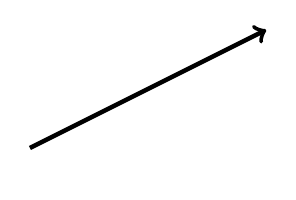
\begin{tikzpicture}
\draw[white] (0,0) -- (0, 0.6);
\draw[->,ultra thick] (0,0.3) --(3,1.8);
\end{tikzpicture}} 
     
\begin{lstlisting}
\smash{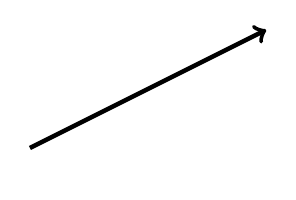
\begin{tikzpicture}
\draw[white] (0,0) -- (0, 0.6);
\draw[->,ultra thick] (0,0.3) --(3,1.8);
\end{tikzpicture}} 
\end{lstlisting}
\end{frame}

\begin{frame}[fragile]{the ``in class task''\magicPage}

This 
was produced by 
\begin{lstlisting}
\tikz[baseline]\node[anchor=base,draw=red,rounded corners,inner xsep=1ex,inner ysep =0.75ex, bottom color=red!20, top color=red!10]{In class task};
\end{lstlisting}
     
\end{frame}

\begin{frame}[fragile]{``Common belief''\magicPage}\relax
     \begin{center}
        \begin{tikzpicture}
             \node[align=center] (0,0) {
             \huge \LaTeX\ is only for use\\ \huge  in academic area
             };
             \uncover<2,3>{\node[rotate=30, bottom color=red!50, top color=red!50] (0,0) {\Huge WRONG}};
        \end{tikzpicture}
         
    \end{center}
    
\pause\pause was produce by 
\begin{lstlisting}
\begin{tikzpicture}
\node[align=center] (0,0) {
\huge \LaTeX\ is only for use\\ \huge  in academic area
};
\uncover<2,3>{\node[rotate=30, bottom color=red!50, top color=red!50] (0,0) {\Huge WRONG}};
\end{tikzpicture}
\end{lstlisting}

    
\end{frame}

